\documentclass[12pt, letterpaper]{article}
\usepackage[utf8]{inputenc}
\usepackage{amsfonts, amsmath, amssymb}
\makeatletter
\makeatother
\usepackage[hidelinks]{hyperref}
\usepackage{comment}
\usepackage{fullpage}
\usepackage[english]{babel}
\usepackage{pdfpages}
\usepackage{tikz}
\usepackage{graphicx}
\usepackage[colorinlistoftodos]{todonotes}
\usepackage[linesnumbered]{algorithm2e}
\usepackage{tabularx}
\usepackage{url}
\usepackage{hyperref}
\hypersetup{colorlinks=true}
\usepackage{multirow}
\usepackage[margin=0.5in]{geometry}
\usepackage[english]{babel}
\usepackage{mathtools}
\usepackage{booktabs}
\usepackage{physics}
\usepackage{enumitem}

\usepackage[thmmarks, thref]{ntheorem}

\theoremstyle{nonumberplain}
\theorembodyfont{\upshape}
\theoremseparator{.}
\theoremsymbol{\ensuremath{\square}}
\theoremsymbol{\ensuremath{\blacksquare}}
\newtheorem{sol}{Solution}
\theoremseparator{. ---}
\theoremsymbol{\mbox{\texttt{;o)}}}
\newtheorem{varsol}{Solution (variant)}

\DeclarePairedDelimiter\ceil{\lceil}{\rceil}
\DeclarePairedDelimiter\floor{\lfloor}{\rfloor}

\usetikzlibrary{matrix}
\setlength{\marginparwidth}{2cm} 

\title{MATH 4640 Numerical Analysis - HW 2 Solutions}

\author{Austin Barton}

\begin{document}
\maketitle

\vspace{2em}

\hspace{18pt}\textbf{Problem 1:} \medskip
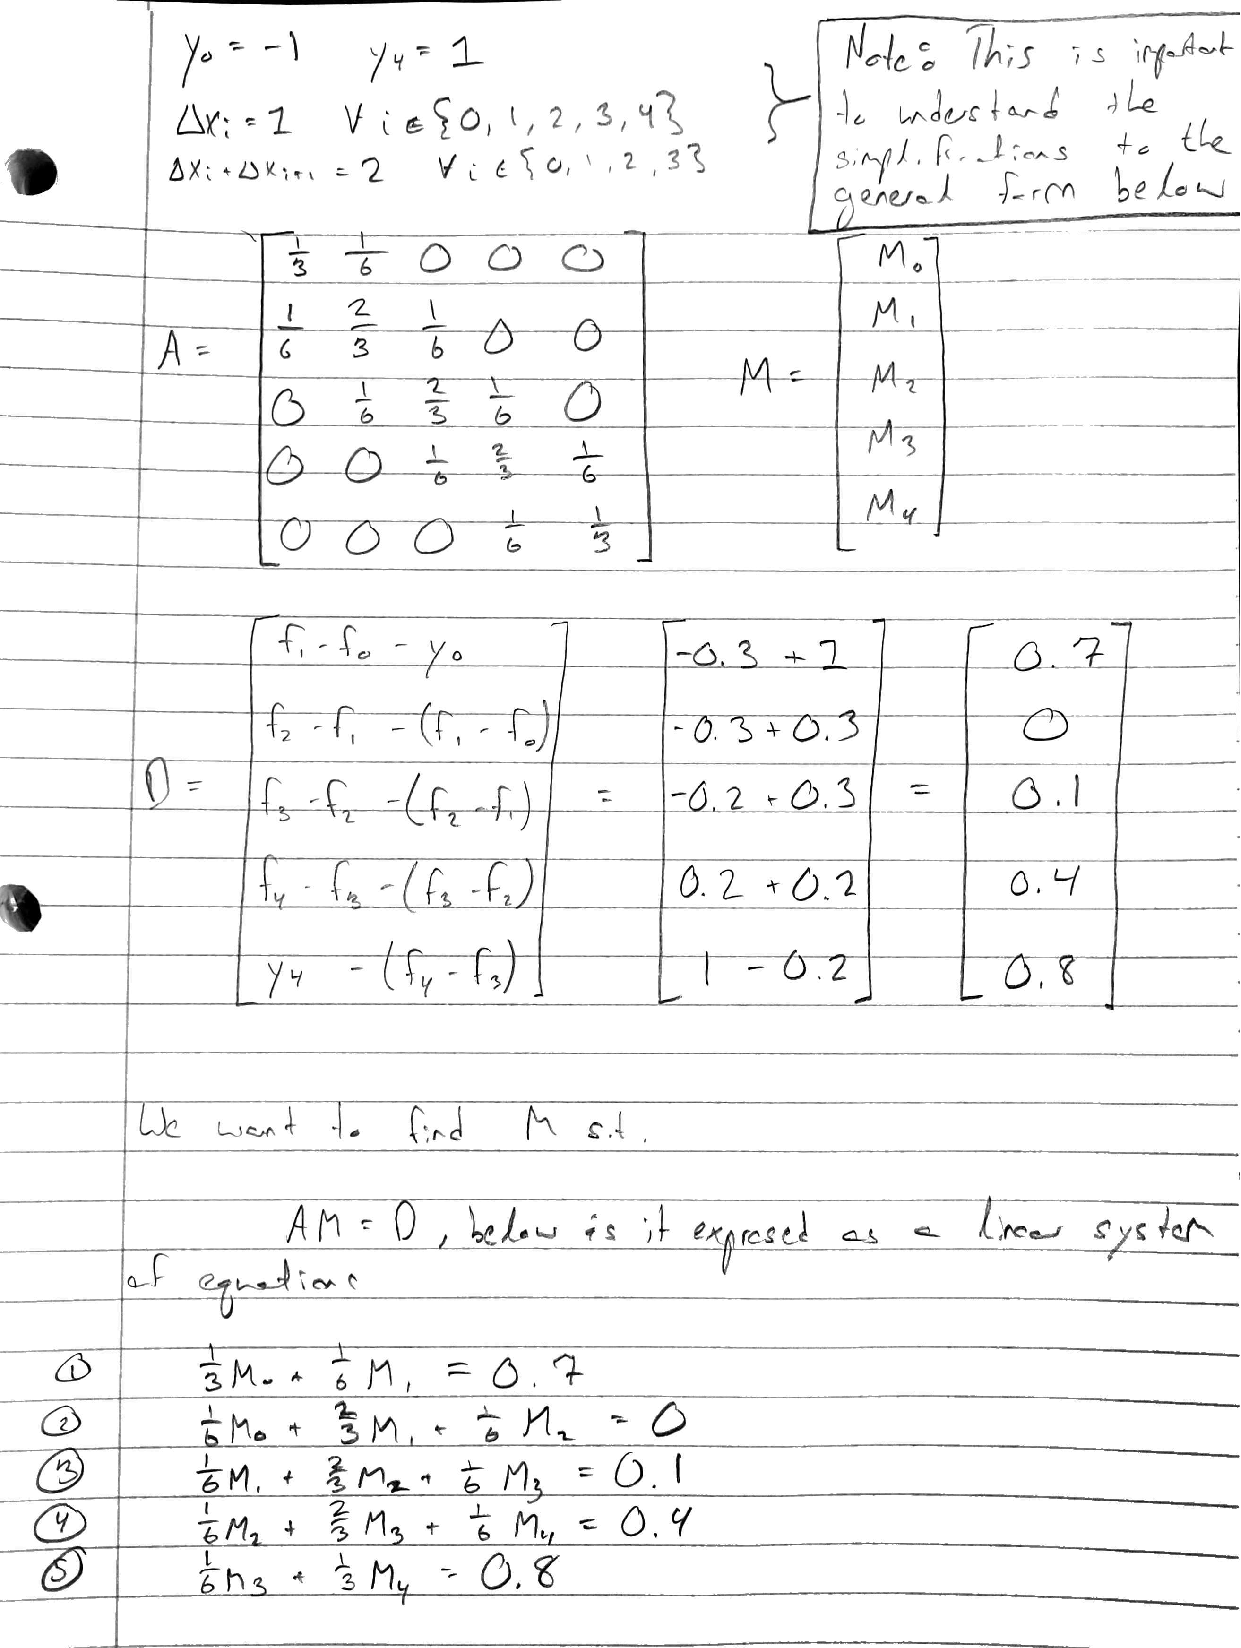
\includepdf[pages=-, scale=0.85]{numhw2q1.pdf}

\hspace{18pt}\textbf{Problem 2:} \medskip
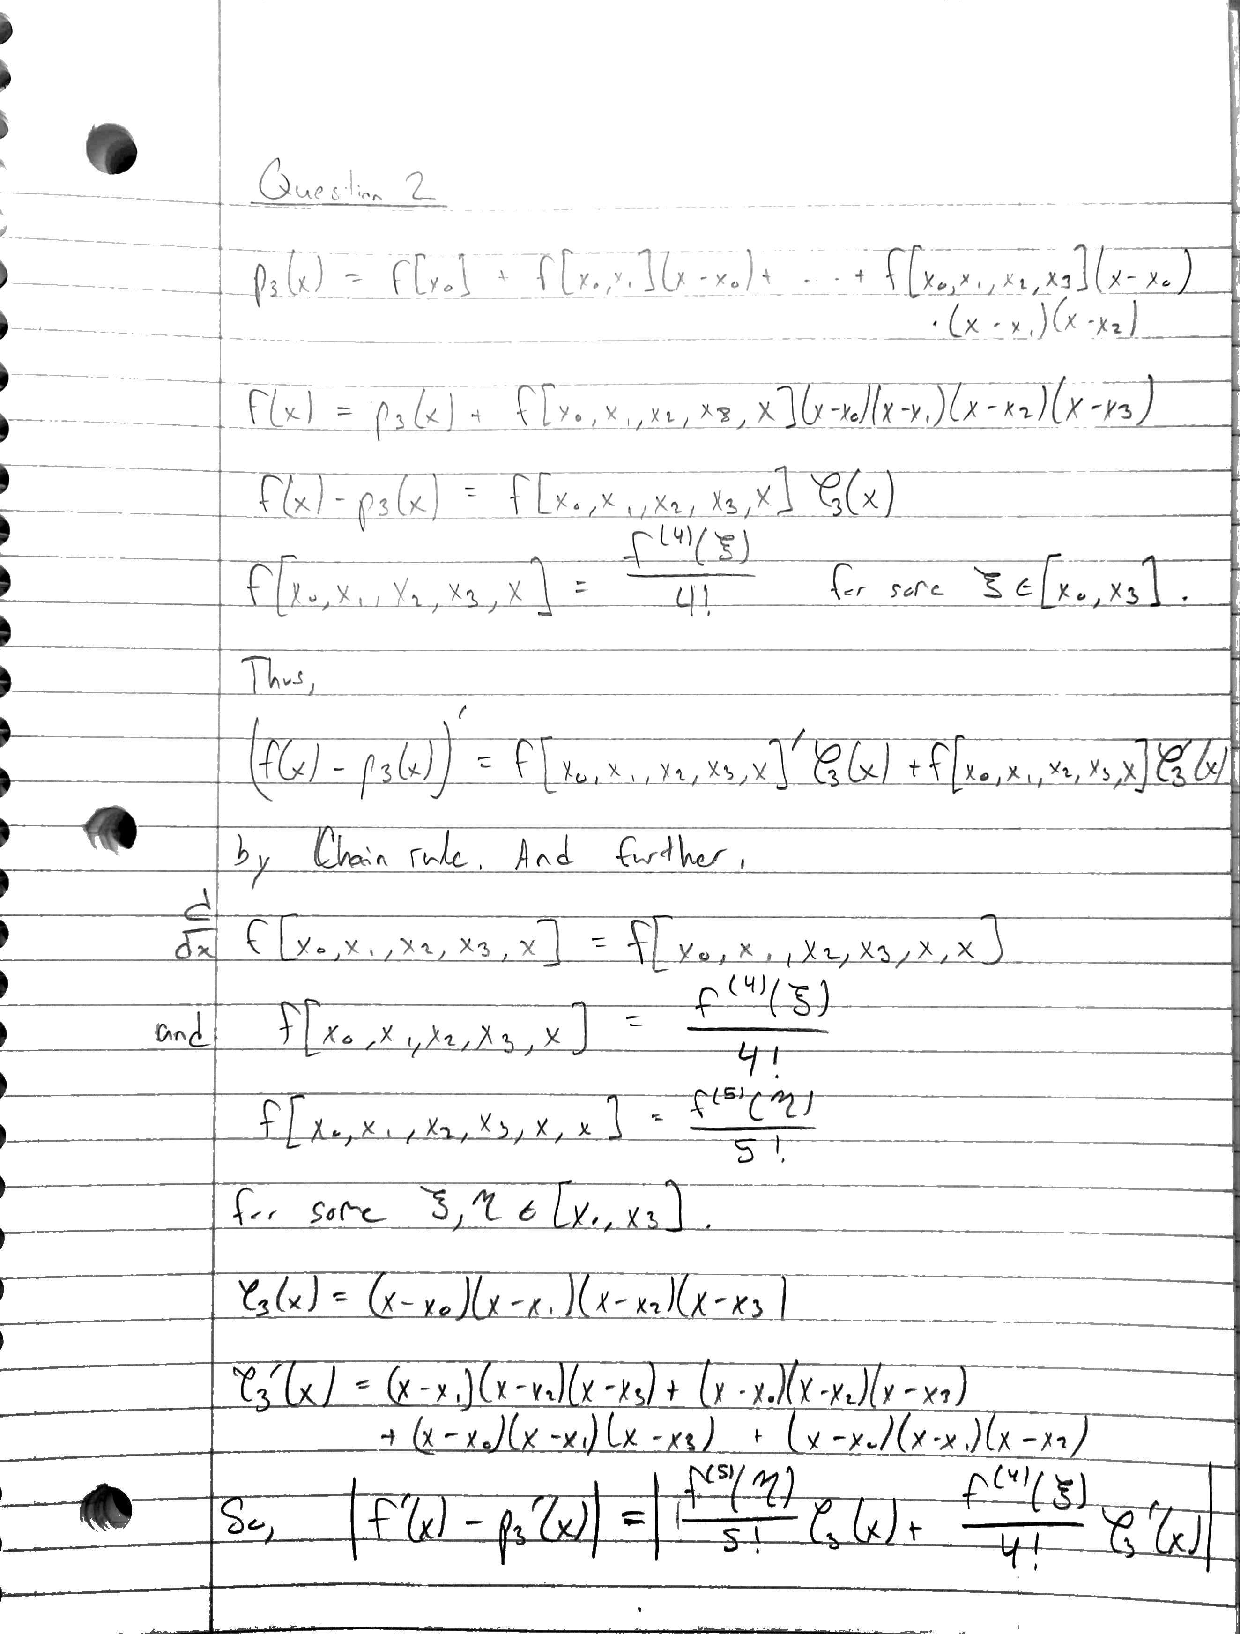
\includepdf[pages=-, scale=0.85]{numhw2q2.pdf}

\hspace{18pt}\textbf{Problem 3:} \medskip
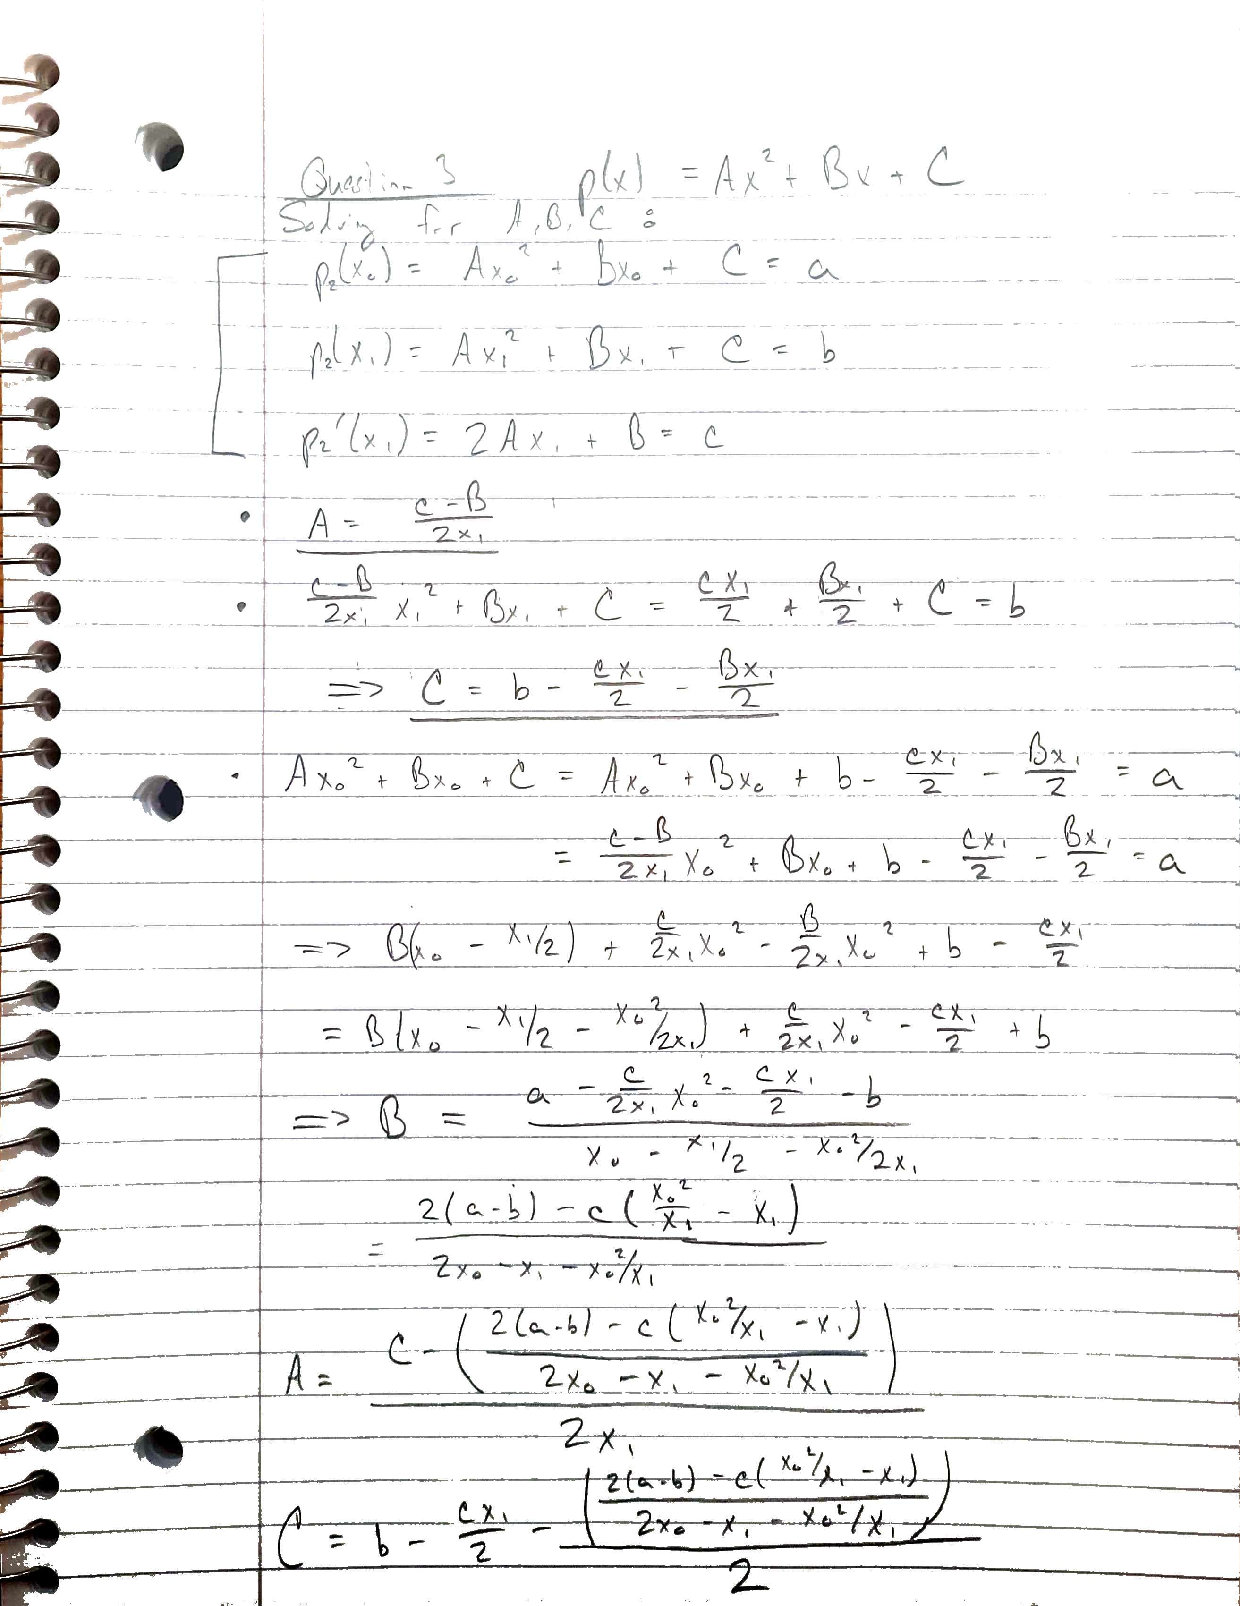
\includepdf[pages=-, scale=0.85]{numhw2q3.pdf}

\hspace{18pt}\textbf{Problem 4:} \medskip

Figures 1-3 show the algorithms of DivDif and Interpolate implemented in Rust, using these algorithms on the data from the problem, and the output of the code when executed. The coefficients obtained from the DivDif algorithm are: $f[x_0] = 7, f[x_0, x_1] = -5, f[x_0, x_1, x_2] = 2, f[x_0, x_1, x_2, x_3] = -2/3, f[x_0, x_1, x_2, x_3, x_4] = 0.29167, f[x_0, x_1, x_2, x_3, x_4, x_5] = -0.125$.

In the output is a test of the Interpolate algorithm on values within the interval of $[-2, 3]$, including interpolated points and not interpolated points, and some points outside of the interval.

\begin{figure}[!htbp]
	\centering
	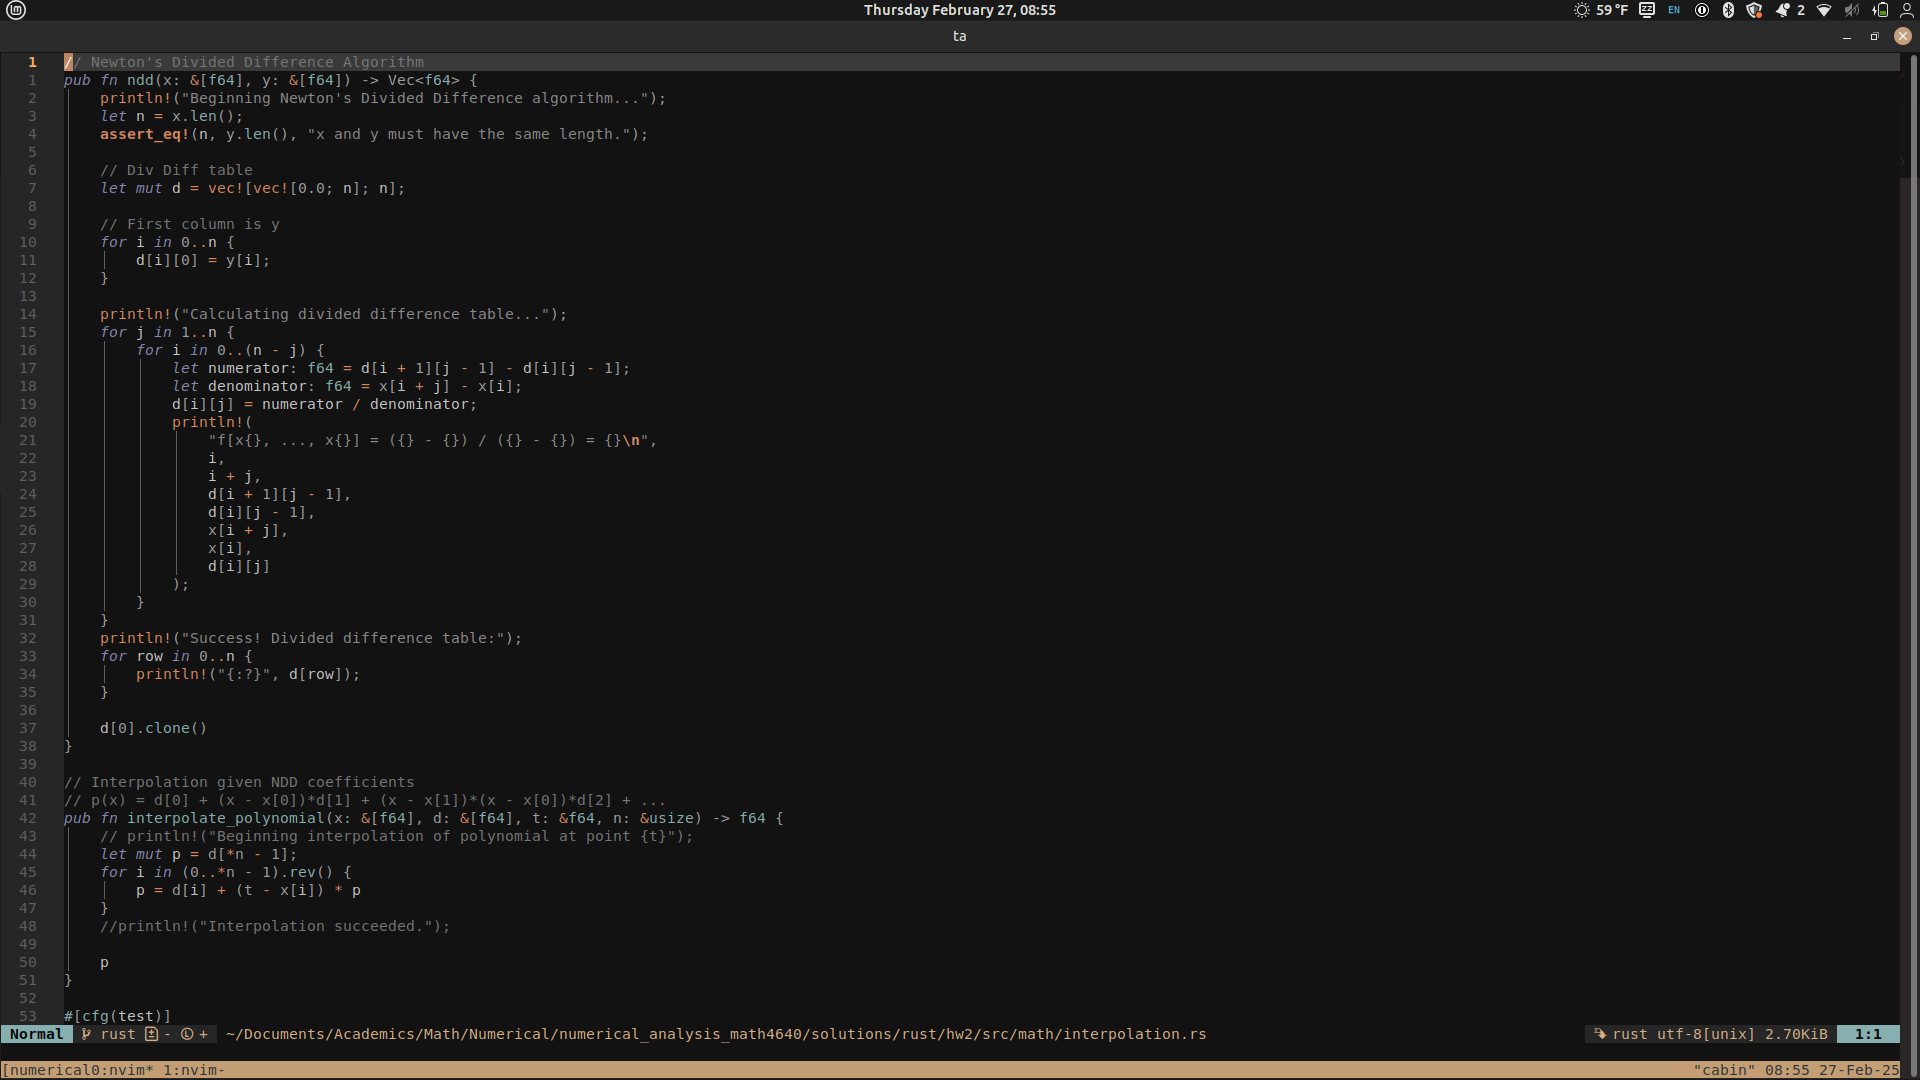
\includegraphics[width=0.8\textwidth]{ndd_and_interpolate_screenshot.png}
	\caption{Screenshot of code for the Newton's Divided Difference (NDD/DivDif) algorithm (upper) and the Interpolate using the NDD coefficients (lower).}
\end{figure}

\begin{figure}[!htbp]
	\centering
	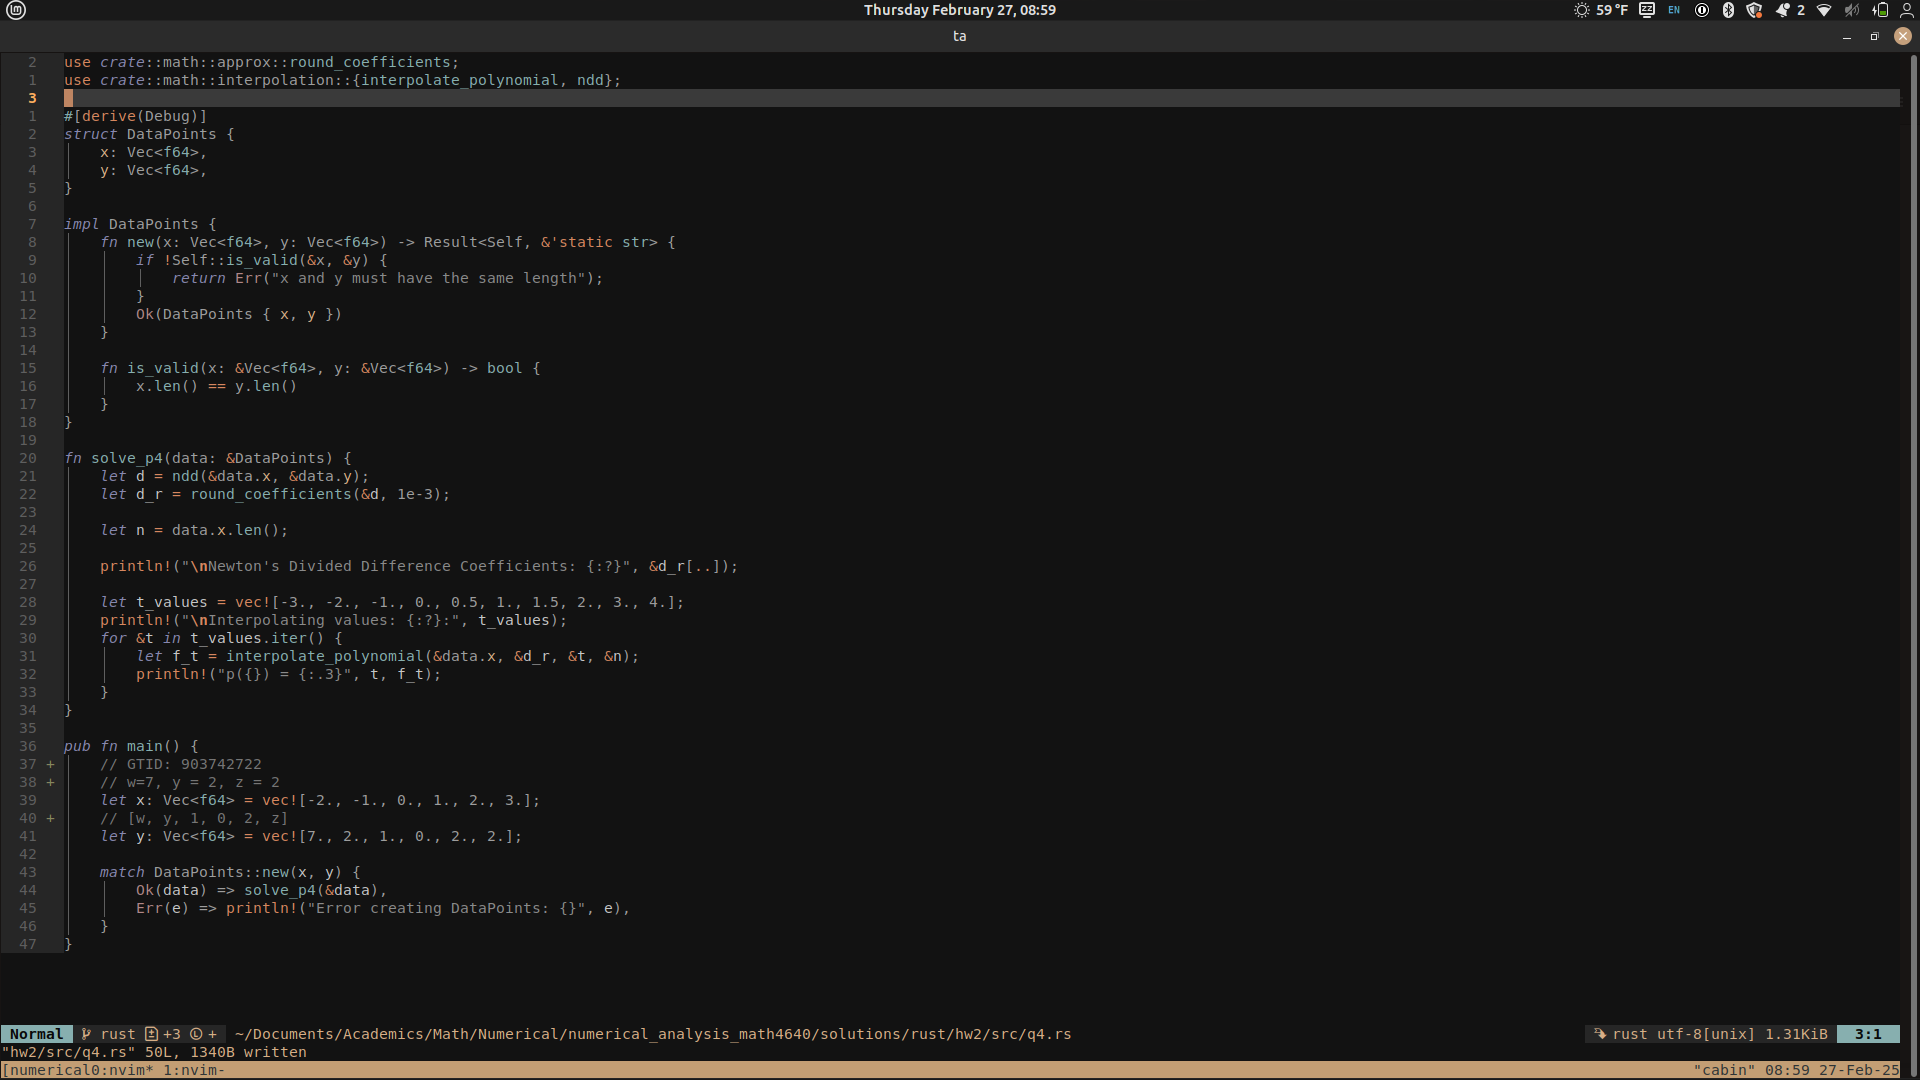
\includegraphics[width=0.8\textwidth]{numhw2q4.png}
	\caption{Screenshot of code using the DivDif and Interpolate algorithms. See Figure 1 for implementation of such algorithms.}
\end{figure}

\begin{figure}[!htbp]
	\centering
	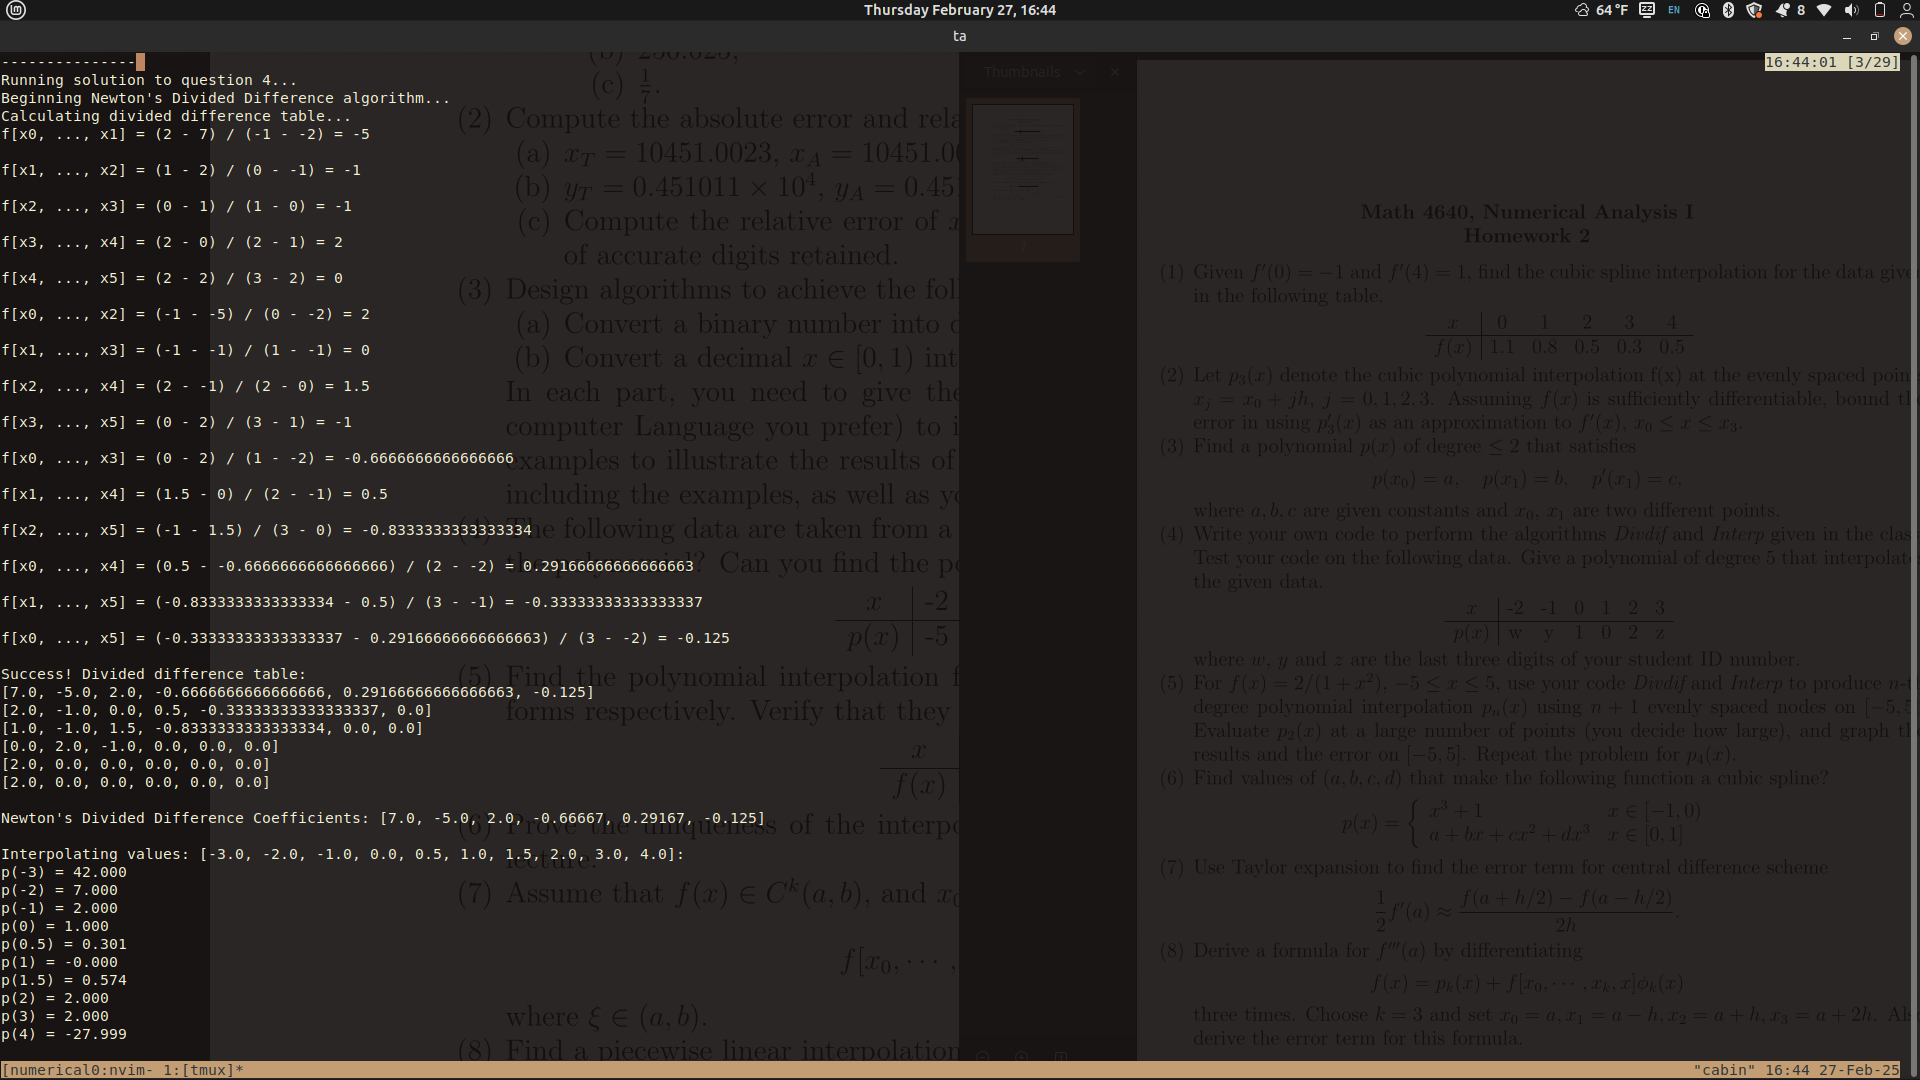
\includegraphics[width=0.8\textwidth]{numhw2q4_output.png}
	\caption{Screenshot of output from code ran in Figure 2. You can run this code for yourself to verify. Documentation in README file with instructions if needed.}
\end{figure}
\clearpage

\hspace{18pt}\textbf{Problem 5:} \medskip

Solution shared below in Figures 3, 4, 5, 6. Figure 5 corresponds to the plot for degree 2 and Figure 6 corresponds to plot for degree 4. The algorithms used are shown above in Figure 1 implemented in Rust.

\begin{figure}[!htbp]
	\centering
	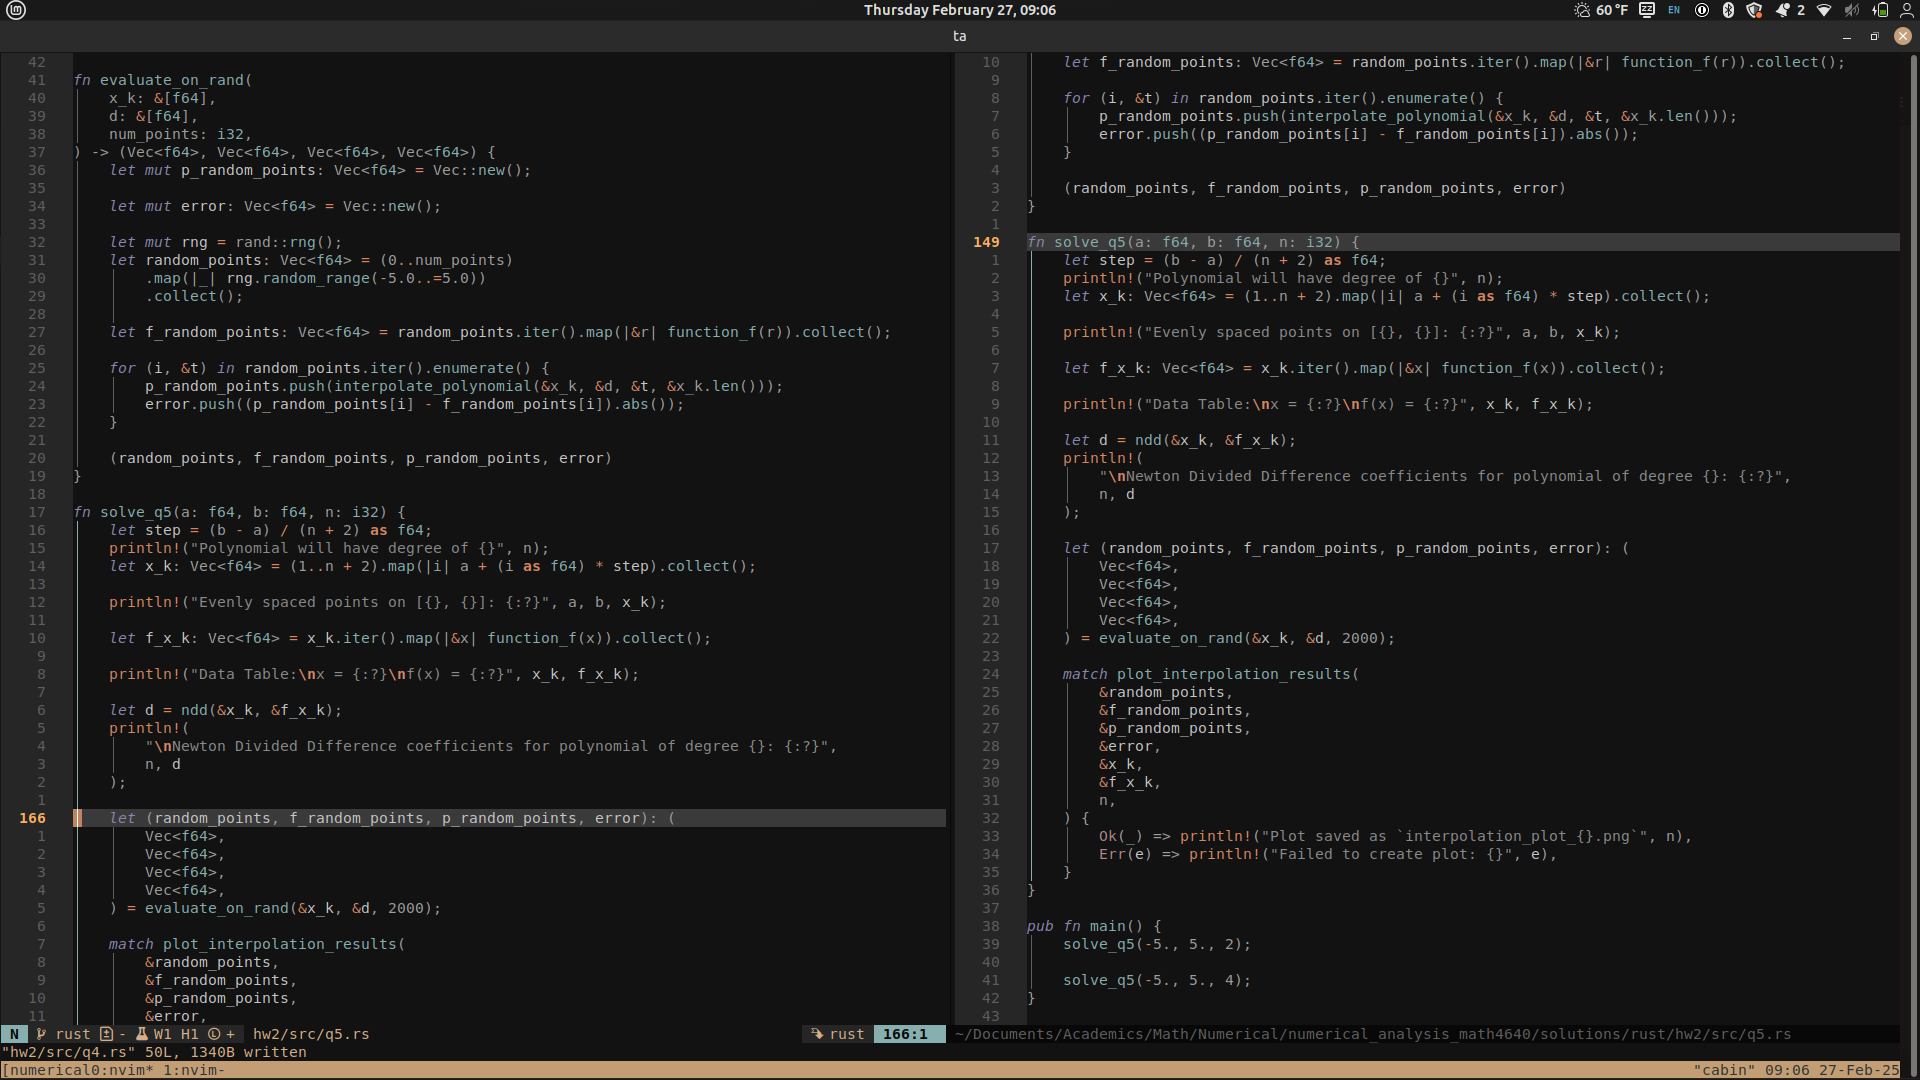
\includegraphics[width=0.8\textwidth]{numhw2q5.png}
	\caption{Screenshot of code using DivDif and Interpolate algorithms. See Figure 1 for implementations of such algorithms.}
\end{figure}

\begin{figure}[!htbp]
	\centering
	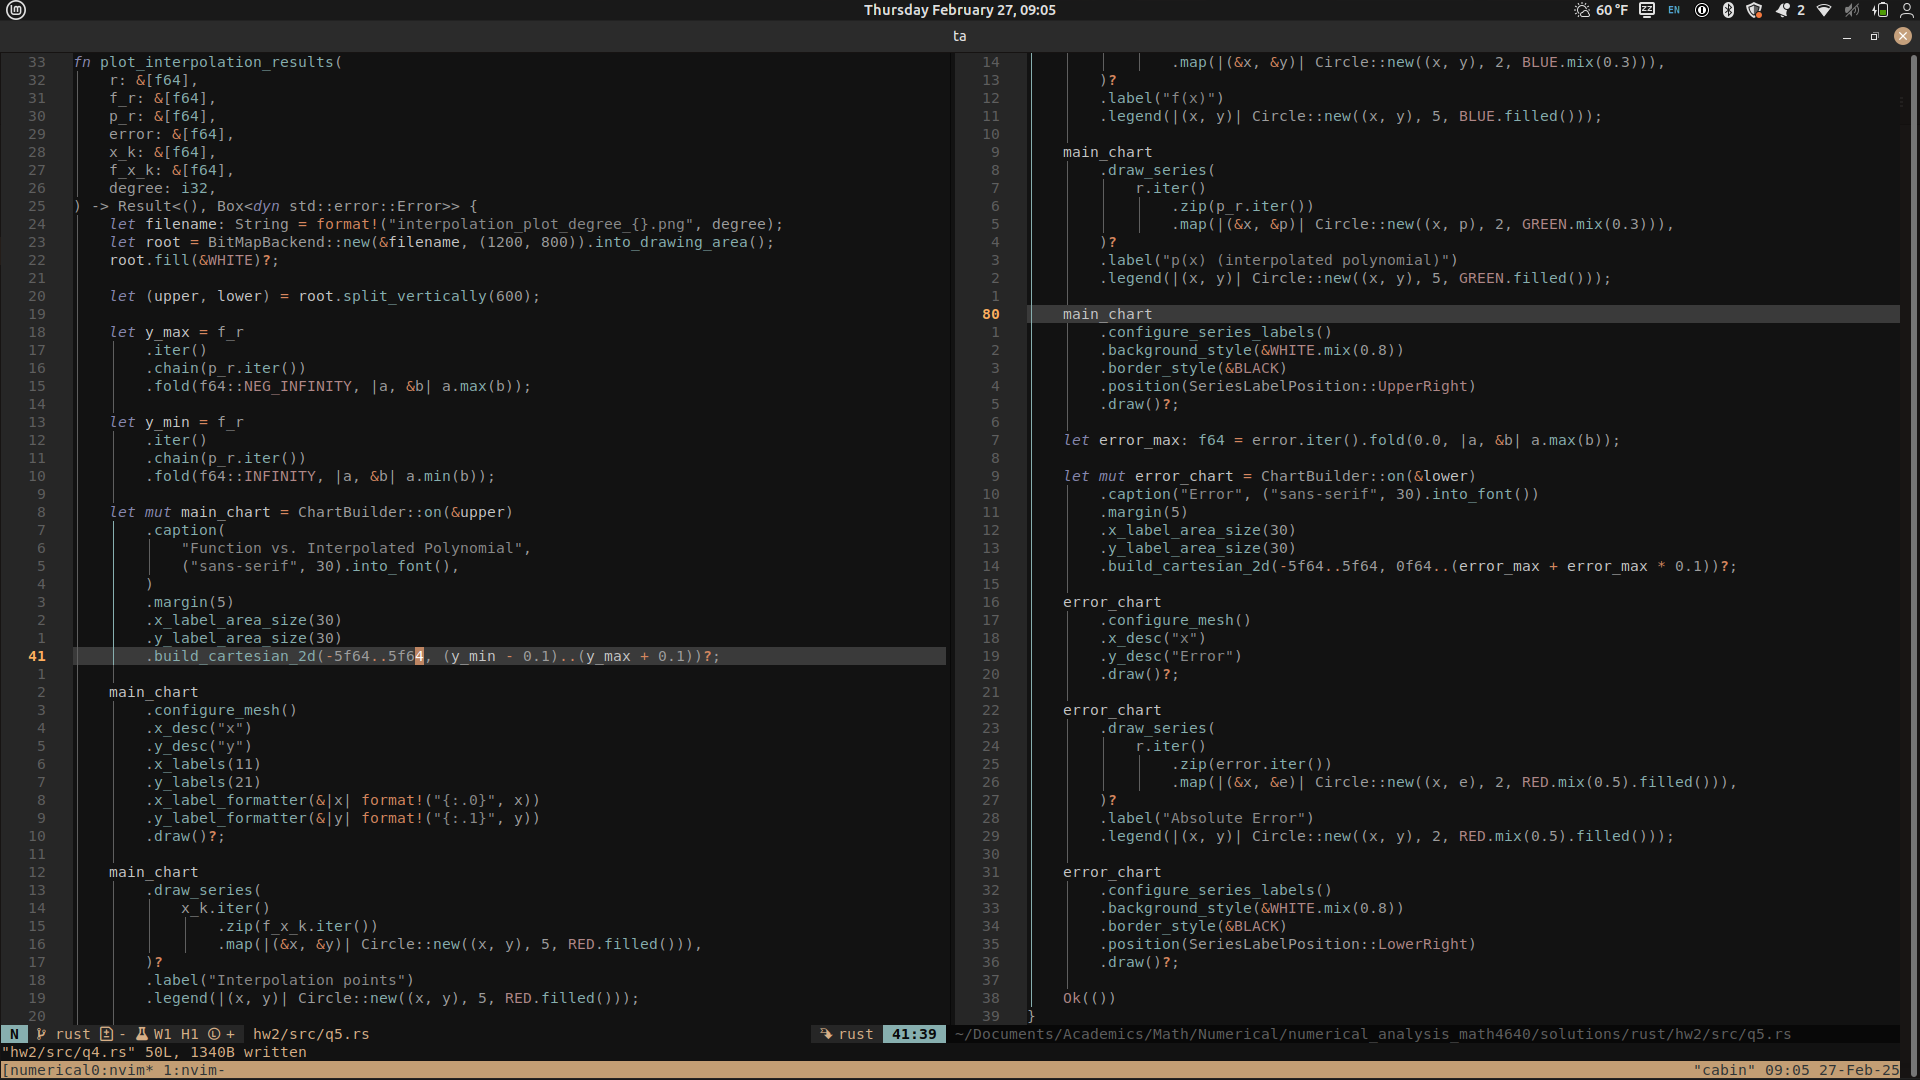
\includegraphics[width=0.8\textwidth]{numhw2q5_plotfunction.png}
	\caption{Screenshot of code plotting the true function, the interpolated polynomial, the interpolated points, and the error between the interpolated polynomial and true function.}
\end{figure}

\begin{figure}[!htbp]
	\centering
	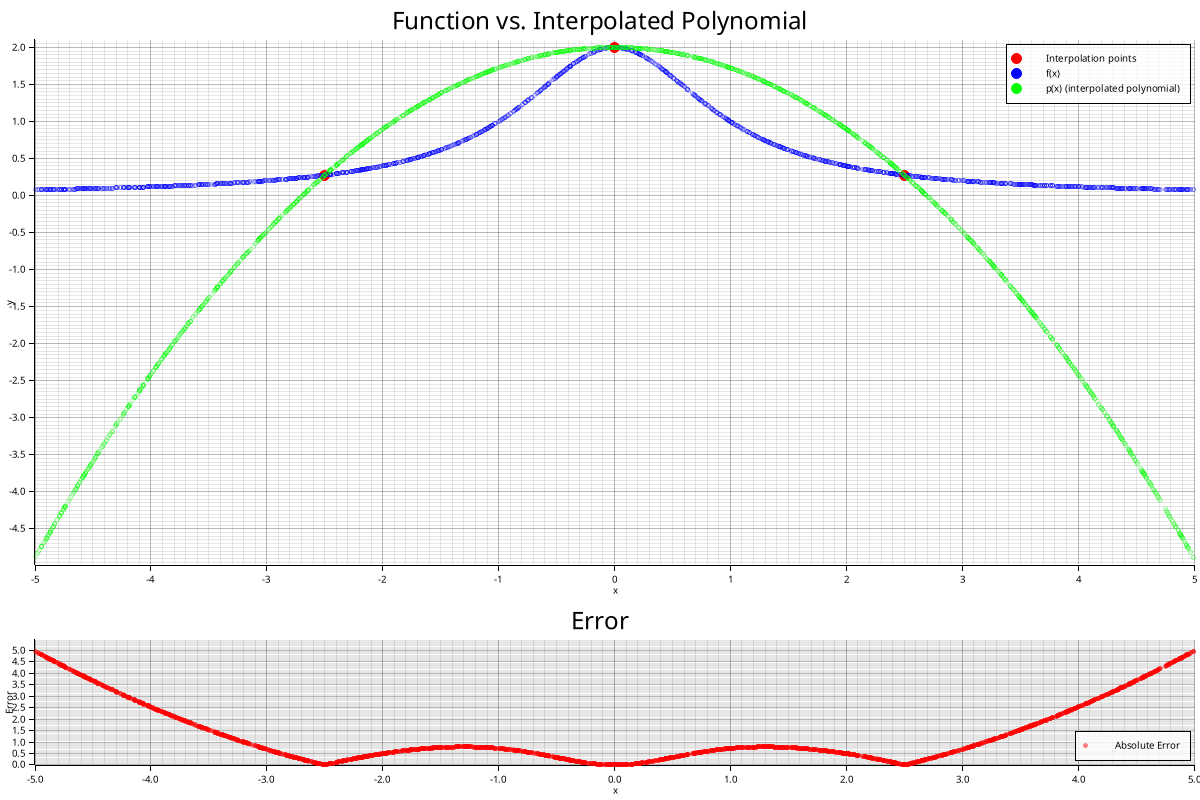
\includegraphics[width=0.8\textwidth]{interpolation_plot_degree_2.png}
	\caption{Plot for degree 2 polynomial and error.}
\end{figure}

\begin{figure}[!htbp]
	\centering
	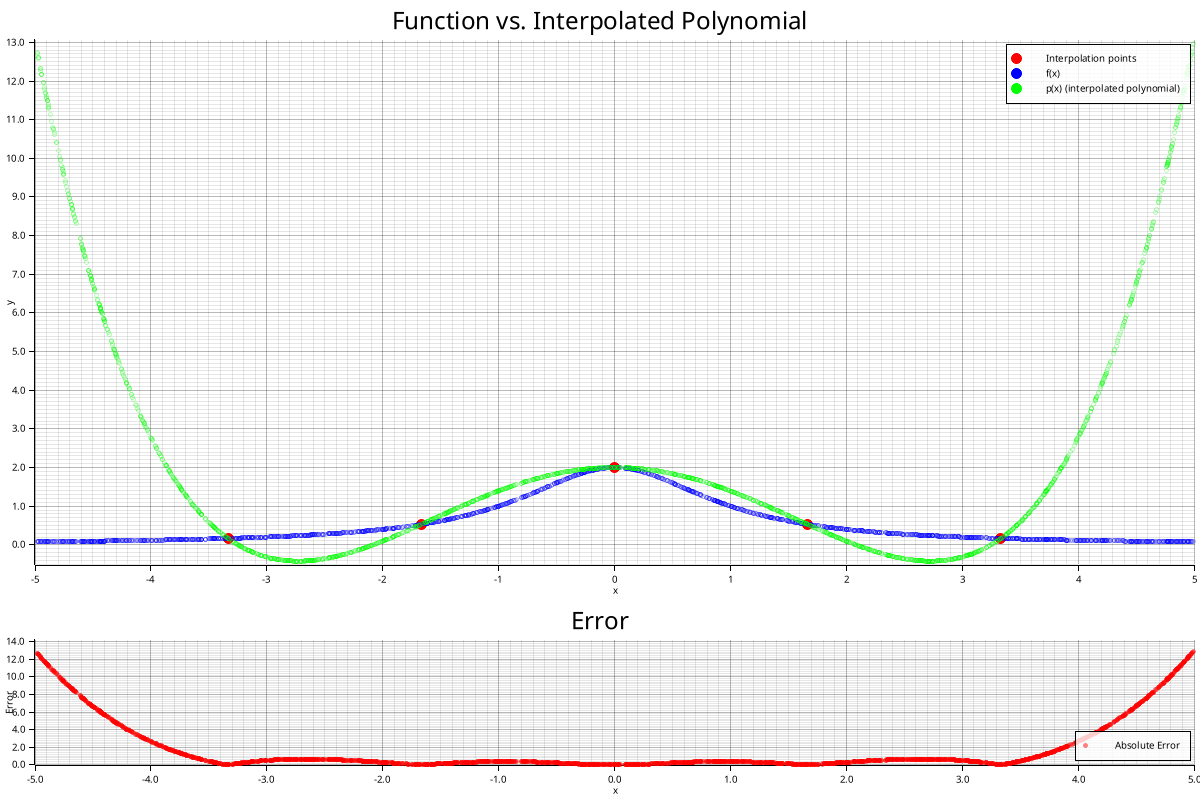
\includegraphics[width=0.8\textwidth]{interpolation_plot_degree_4.png}
	\caption{Plot for degree 4 polynomial and error.}
\end{figure}

\clearpage

\hspace{18pt}\textbf{Problem 6:} \medskip
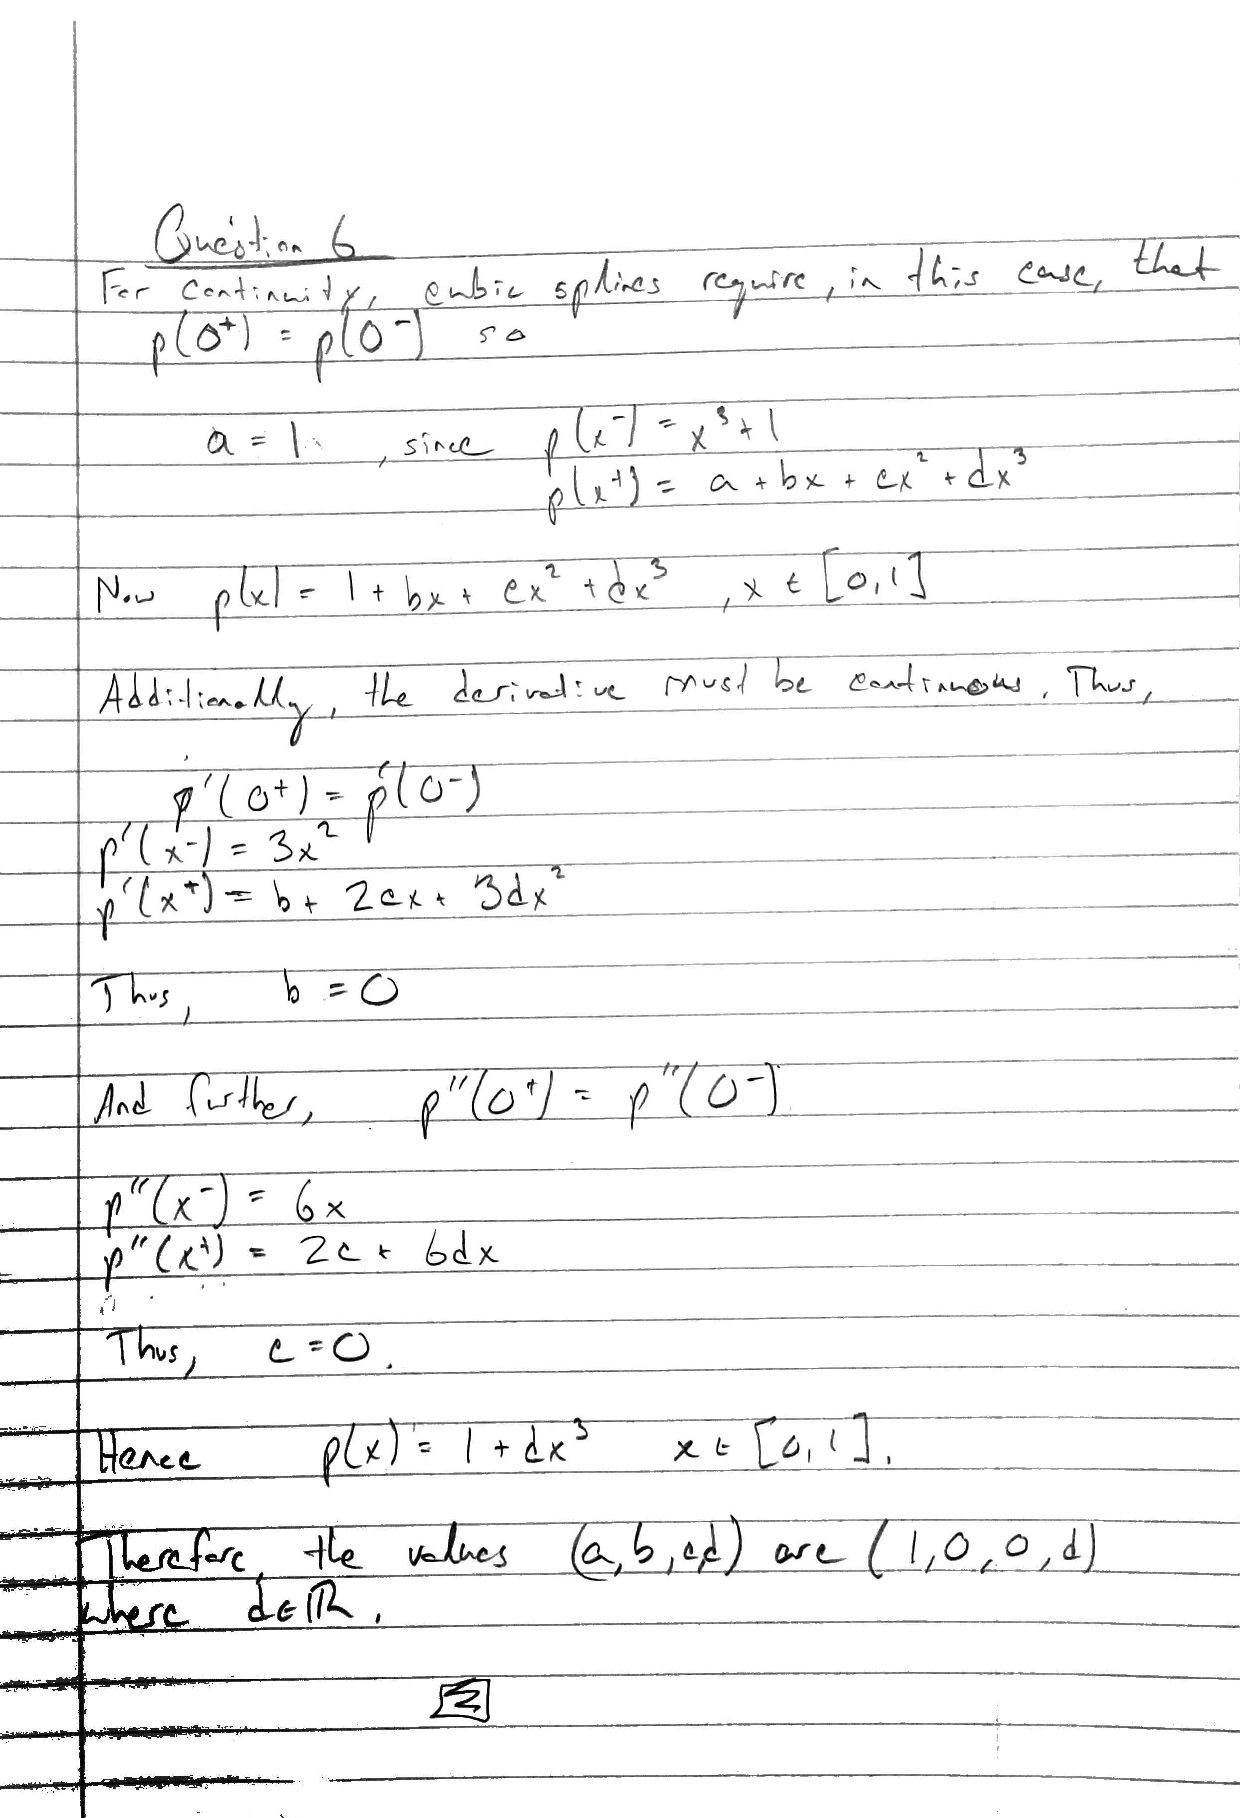
\includepdf[pages=-, scale=0.85]{numhw2q6.pdf}

\hspace{18pt}\textbf{Problem 7:} \medskip
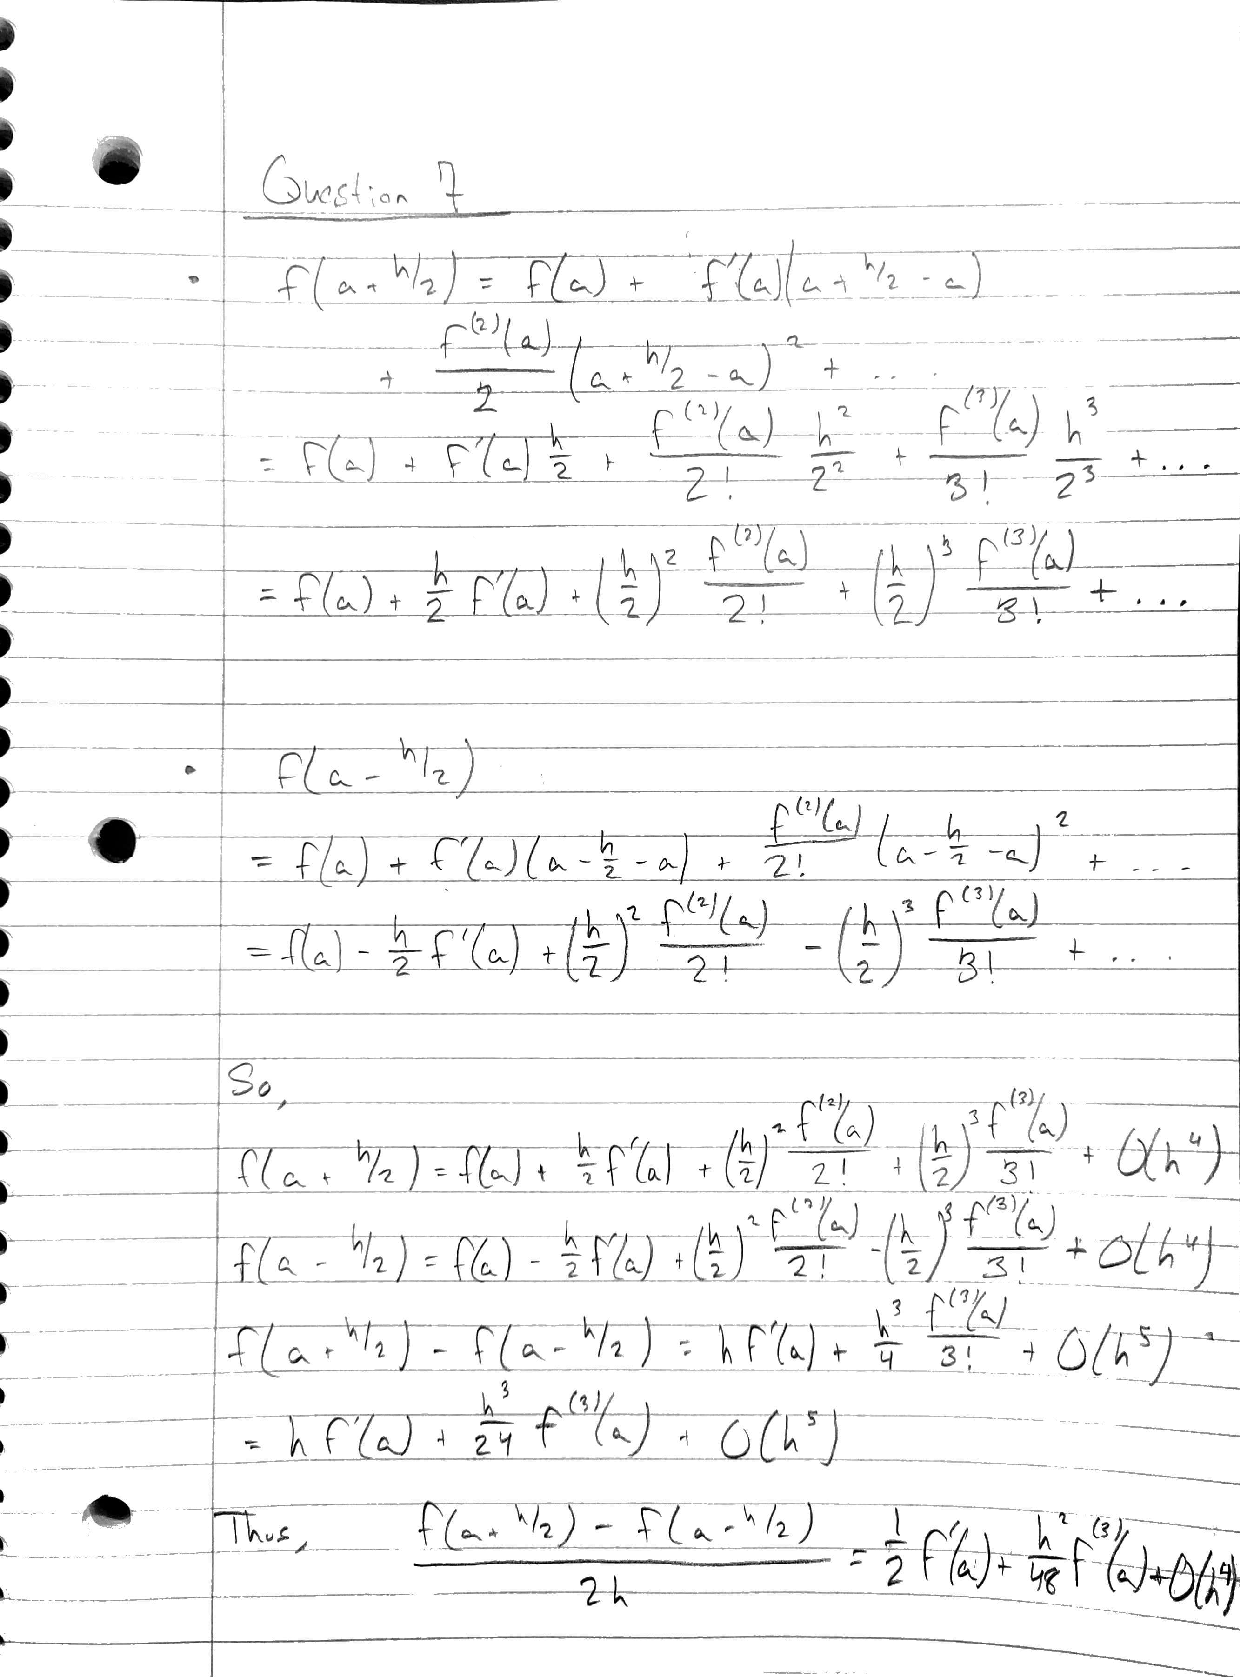
\includepdf[pages=-, scale=0.85]{numhw2q7.pdf}

\hspace{18pt}\textbf{Problem 8:} \medskip
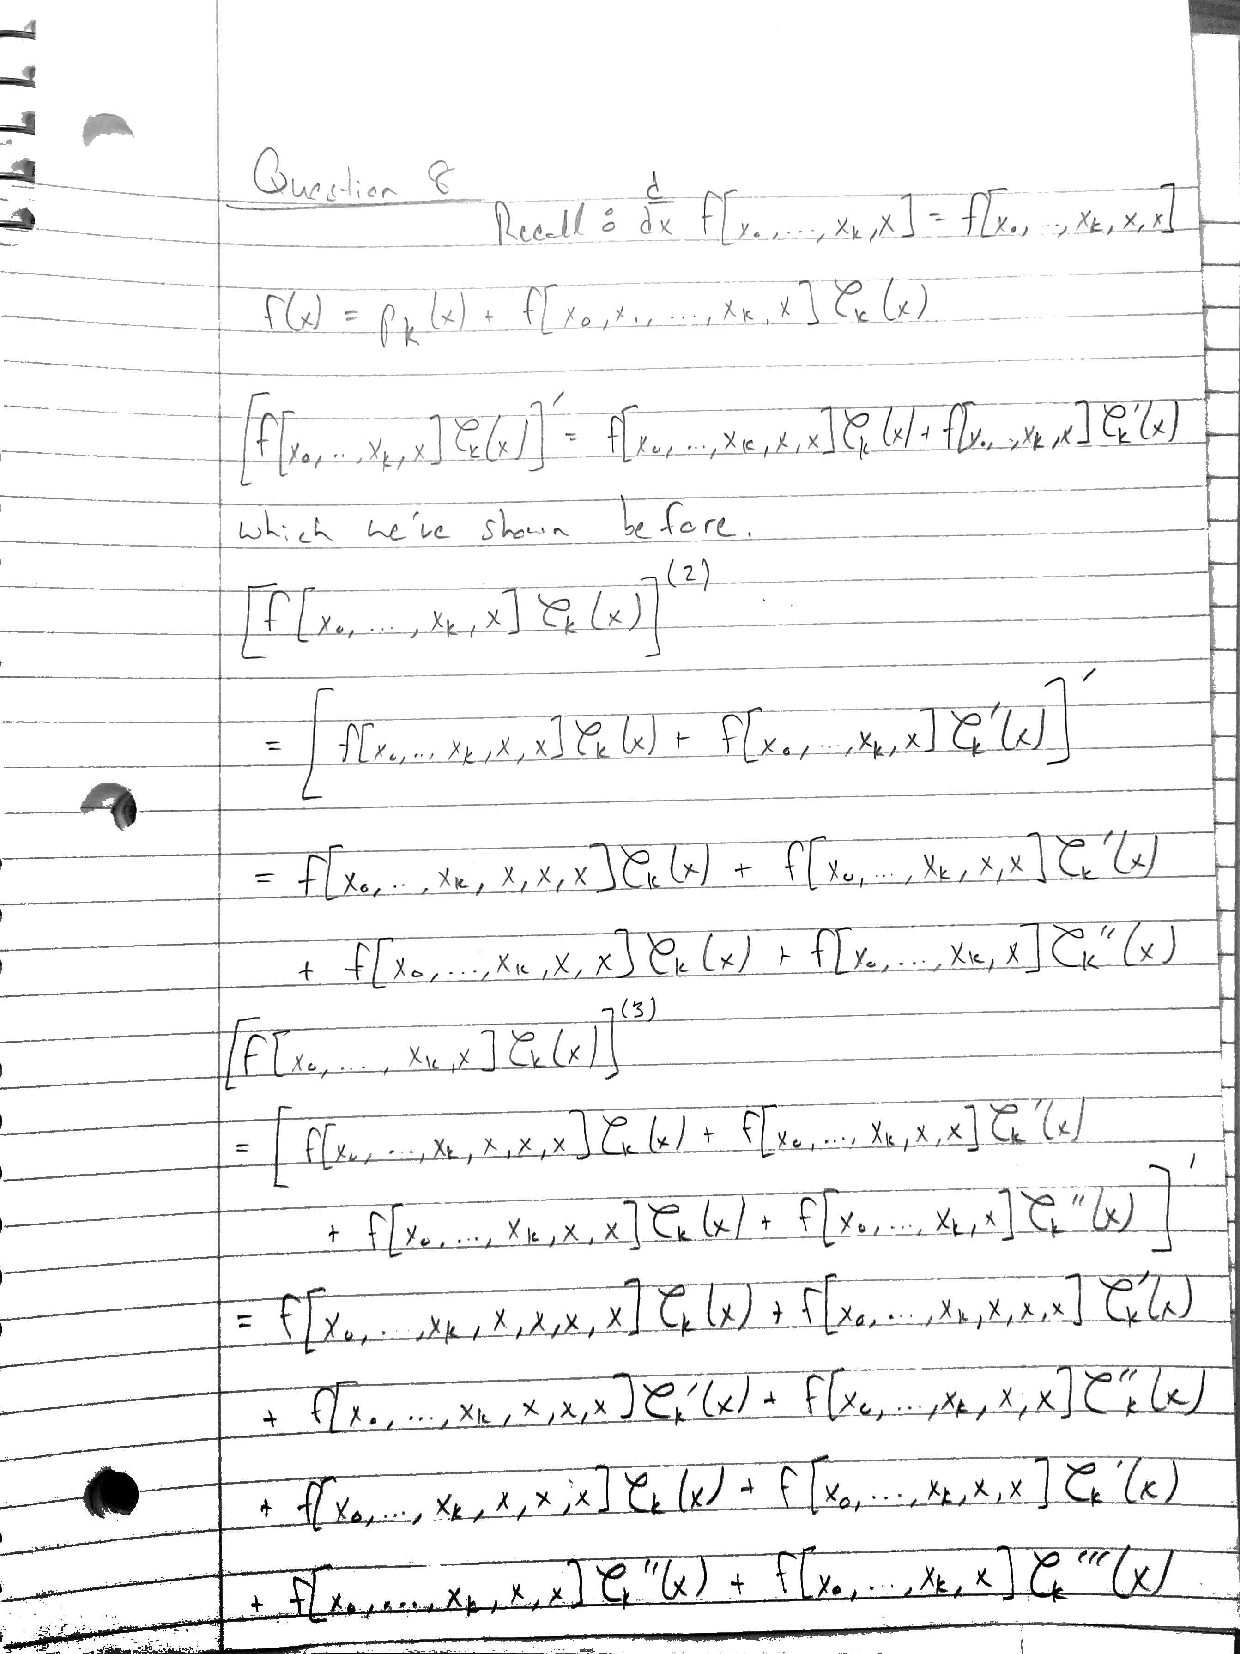
\includepdf[pages=-, scale=0.85]{numhw2q8.pdf}

\end{document}
